This chapter describes once, canonically, the hardware, firmware,
software and measurement tooling used by every experiment reported in
this paper. Chapters that present a specific optimisation --- the
SDRAM-to-tensor eDMA memcpy (\url{memcpy.md}) and the glitch-free
dual-camera switch (\url{cam_switch.md}) --- refer back to this
description rather than repeating it. The same configuration is used
end-to-end across all reported sessions; departures are flagged
explicitly in the individual result tables.

\begin{center}\rule{0.5\linewidth}{0.5pt}\end{center}

\section{1. Hardware platform}\label{hardware-platform}

The device under test is a Coral Dev Board Micro carrying the
custom-designed \textbf{SentAI} daughter-board revision v1.0. The
relevant subsystems of this stack are summarised below.

{\def\LTcaptype{none} % do not increment counter
\begin{longtable}[]{@{}
  >{\raggedright\arraybackslash}p{(\linewidth - 4\tabcolsep) * \real{0.3333}}
  >{\raggedright\arraybackslash}p{(\linewidth - 4\tabcolsep) * \real{0.3333}}
  >{\raggedright\arraybackslash}p{(\linewidth - 4\tabcolsep) * \real{0.3333}}@{}}
\toprule\noalign{}
\begin{minipage}[b]{\linewidth}\raggedright
Subsystem
\end{minipage} & \begin{minipage}[b]{\linewidth}\raggedright
Component
\end{minipage} & \begin{minipage}[b]{\linewidth}\raggedright
Parameters
\end{minipage} \\
\midrule\noalign{}
\endhead
\bottomrule\noalign{}
\endlastfoot
MCU & NXP i.MX RT1176 crossover & Cortex-M7 @ 800 MHz + Cortex-M4
co-processor (M4 is idle throughout our measurements) \\
On-chip AI accelerator & Google EdgeTPU & internal USB 2.0 bus, Mode 3
(\texttt{kMax}) requested by \texttt{sentai.tpu.load()} \\
External SDRAM & On-module SEMC SDR-SDRAM & 16 MB @ 166 MHz, accessible
via the SEMC controller \\
On-chip memory & OCRAM / DTCM / ITCM & 1.25 MB / 256 KB / 256 KB \\
External flash & Octal-SPI NAND + NOR & NAND hosts the LittleFS user
partition (firmware + \texttt{/diags/} data + \texttt{/lib/diag/}
package) \\
Camera 0 (front) & OV5640-based coralmicro module & 1280×720 native, 30
fps streaming (see §3) \\
Camera 1 (back) & OV5640-based coralmicro module & 1280×720 native, 30
fps streaming \\
Camera MUX & Analogue switch on the shared MIPI-CSI2 lane &
GPIO-controlled (\texttt{kCamMux}); GPIO polarity canonicalised in
\href{../../../libs/camera/cam_mux.h}{cam\_mux.h} \\
Host link & USB-C to Linux workstation & CDC-ACM (REPL) + CDC-NCM (IP
10.0.0.1) simultaneously; see \url{usb.md} \\
Power & USB-C bus-powered & no separate supply; thermal envelope within
the 3-second experiment windows \\
\end{longtable}
}

The only dual-sensor hardware constraint that matters for
interpretation: \textbf{the two OV5640 sensors share a single MIPI-CSI2
lane through an analogue MUX}. There is no hardware sync pin wired
between them (no FSIN master/slave), so their internal frame clocks
drift independently. Every measurement of ``switch cost'' in this work
is a measurement against \emph{that} topology, not against a
two-receiver SoC.

\begin{center}\rule{0.5\linewidth}{0.5pt}\end{center}

\section{2. Firmware stack}\label{firmware-stack}

{\def\LTcaptype{none} % do not increment counter
\begin{longtable}[]{@{}
  >{\raggedright\arraybackslash}p{(\linewidth - 2\tabcolsep) * \real{0.5000}}
  >{\raggedright\arraybackslash}p{(\linewidth - 2\tabcolsep) * \real{0.5000}}@{}}
\toprule\noalign{}
\begin{minipage}[b]{\linewidth}\raggedright
Component
\end{minipage} & \begin{minipage}[b]{\linewidth}\raggedright
Version / parameters
\end{minipage} \\
\midrule\noalign{}
\endhead
\bottomrule\noalign{}
\endlastfoot
Firmware project & \texttt{examples/sentai\_runtime/}, build
\textbf{\#640+} at the time of the final post-refactor session
(\texttt{s045\_e18\_post\_refactor}) \\
Linker script & \texttt{MIMXRT1176xxxxx\_cm7\_ram\_mp.ld} (text and
rodata in flash, working set in SDRAM) \\
RTOS & FreeRTOS 10.x (CMSIS M7 build, 1 ms tick) \\
USB stack & NXP USB device driver, CDC-ACM + CDC-NCM simultaneously (MSC
only in ``storage mode''; see \url{usb.md}) \\
HTTP server & lwIP httpd with custom \texttt{FsOpenCustom} /
\texttt{FsCloseCustom} in \href{../sentai_httpd.cc}{sentai\_httpd.cc};
LS requests route through a dedicated lfs\_task --- see \url{lfs.md}
§4.2 build \#633 for the rationale \\
MicroPython runtime & stable embed port under
\texttt{third\_party/micropython/ports/embed}; GC heap \textbf{512 KB}
in \texttt{.sdram\_bss} \\
EdgeTPU driver & Coral \texttt{EdgeTpuManager} with per-model package
cache \\
Camera driver & NXP \texttt{fsl\_ov5640.c} + \texttt{camera.cc}, with
the custom additions documented in \url{cam_switch.md} (flip-on-EOF ISR,
ratio scheduler) \\
Watchdog & WDOG1 hardware @ 30 s; software activity watchdog with 60 s
warn / 120 s dead thresholds --- \url{watchdog.md} \\
Persistent diagnostic store & LittleFS user partition, \texttt{/diags/}
and \texttt{/lib/diag/} subtrees \\
\end{longtable}
}

The firmware image for a reported result is identified by
\texttt{build\_version.h} and reflected in every session's
\texttt{summary.txt} (implicit via build date) and in the session name
suffix we chose at the time (e.g.~\texttt{\_post\_refactor}). Major
build transitions called out in the results tables:

{\def\LTcaptype{none} % do not increment counter
\begin{longtable}[]{@{}
  >{\raggedright\arraybackslash}p{(\linewidth - 4\tabcolsep) * \real{0.3333}}
  >{\raggedright\arraybackslash}p{(\linewidth - 4\tabcolsep) * \real{0.3333}}
  >{\raggedright\arraybackslash}p{(\linewidth - 4\tabcolsep) * \real{0.3333}}@{}}
\toprule\noalign{}
\begin{minipage}[b]{\linewidth}\raggedright
Transition
\end{minipage} & \begin{minipage}[b]{\linewidth}\raggedright
Build
\end{minipage} & \begin{minipage}[b]{\linewidth}\raggedright
Effect
\end{minipage} \\
\midrule\noalign{}
\endhead
\bottomrule\noalign{}
\endlastfoot
Pre-eDMA CPU memcpy & \#584 or earlier & baseline used as the left-hand
side of \url{memcpy.md} tables \\
eDMA memcpy merged & ≈\#622 & \texttt{sentai.pipeline.dma\_memcpy(0/1)}
A/B flag available at runtime \\
Fix A (atomic snapshot) & \#632 & \url{cam_switch.md} §``Fix A'' \\
Fix B (flip-on-EOF, 30 fps, ratio scheduler) & \#635 &
\url{cam_switch.md} §``Fix B'' \\
LS slow-path (reset-loop fix) & \#633 & \url{lfs.md} §4.2 \\
NASA/JPL review refactor (A1-A7, B1-B4) & \#640 & \url{cam_switch.md}
§``Fix B post-review'' \\
\end{longtable}
}

\begin{center}\rule{0.5\linewidth}{0.5pt}\end{center}

\section{3. Sensor configuration}\label{sensor-configuration}

\subsection{3.1 Native mode}\label{native-mode}

Both OV5640s are driven at \textbf{1280×720 @ 30 fps} in MIPI-CSI2 mode,
with the PLL lookup at
\texttt{s\_ov5640MipiClockConfigs{[}resolution=720P,\ framePerSec=30{]}}:

\begin{verbatim}
pllCtrl1 = 0x21   // SYSTEM_CLK_DIV = 2
pllCtrl2 = 0x54   // PLL multiplier = 84
vfifoCtrl0C = 0x20
pclkDiv = 0x04
pclkPeriod = 0x0a
\end{verbatim}

\texttt{tHsSettle} in the CSI2RX is set to \texttt{0x12} --- the
NXP-recommended value for this (resolution, fps) pair. Attempts to push
to 45 fps (not in the NXP driver lookup) or 60 fps (PLL accepted, CSI2RX
did not lock) were reverted and are documented in the comment block of
\texttt{libs/camera/camera\_support.h}.

\subsection{3.2 Logical resolution}\label{logical-resolution}

The host application requests a logical resolution via
\texttt{sentai.camera.set\_resolution(w,\ h)\ +\ sentai.camera.init(1)}.
The firmware reconfigures the CSI receiver accordingly. Supported pairs
are the union of the NXP driver lookup and the sentai wrapper: 720p,
1080p (limited mode), 640×480 (VGA), 320×240 (QVGA), plus the custom
512×512 target used by the TPU model. Every experiment's \texttt{.txt}
descriptor records the resolution active during that run.

\subsection{3.3 Rotation}\label{rotation}

\texttt{cam0} is configured with a 180° rotation
(\texttt{sentai.camera.rotate(0,\ 180)}) via OV5640 MIRROR H/V registers
at sensor-init time. \texttt{cam1} is unrotated. Rotation does not
change per-frame cost.

\begin{center}\rule{0.5\linewidth}{0.5pt}\end{center}

\section{4. Vision model under test}\label{vision-model-under-test}

The single-class 512×512 model used for every E15-E18 session is:

{\def\LTcaptype{none} % do not increment counter
\begin{longtable}[]{@{}
  >{\raggedright\arraybackslash}p{(\linewidth - 2\tabcolsep) * \real{0.5000}}
  >{\raggedright\arraybackslash}p{(\linewidth - 2\tabcolsep) * \real{0.5000}}@{}}
\toprule\noalign{}
\begin{minipage}[b]{\linewidth}\raggedright
Property
\end{minipage} & \begin{minipage}[b]{\linewidth}\raggedright
Value
\end{minipage} \\
\midrule\noalign{}
\endhead
\bottomrule\noalign{}
\endlastfoot
File &
\texttt{/yolo\_1\_class\_512\_1\_upsample\_512\_inloc\_de\_1024\_la\_P5\_32.tflite} \\
On-flash size & 5 591 680 B (5.33 MB) \\
Input tensor & \texttt{uint8{[}1,\ 512,\ 512,\ 3{]}} --- \textbf{786 432
B}, the buffer at the centre of the eDMA memcpy optimisation \\
Input quantisation & scale = 1/255, zero\_point = 0 \\
Output tensor & \texttt{uint8{[}1,\ 1344,\ 6{]}} --- 8 064 B ---
YOLOv5-enhanced anchor format \\
Output quantisation & scale = 1/255, zero\_point = 0 \\
Output row layout &
\texttt{{[}cx,\ cy,\ w,\ h,\ obj\_conf,\ class\_conf{]}} (normalised
0..1) \\
Architecture & YOLOv5 enhanced, single-upsample at P5/32, 1-class
head \\
TFLite arena & 799 KB used / 8 192 KB available \\
EdgeTPU mode & 3 (\texttt{kMax}), fully compiled for the accelerator (no
CPU fallback) \\
\end{longtable}
}

The earlier pipeline-bring-up sessions (E1-E14 groundwork, listed in
Appendix A of \href{../experiments/README.md}{experiments/README.md})
used \texttt{yolo26n.edgetpu\_1.tflite} --- an 80-class model at 320×320
that partially falls back to CPU. Those sessions are baseline evidence
for the \texttt{\textasciitilde{}6.4\ FPS} floor; they are not presented
as final performance numbers.

\begin{center}\rule{0.5\linewidth}{0.5pt}\end{center}

\section{5. Scene}\label{scene}

All camera-related measurements were captured with a static scene: two
lilac flower arrangements against a pale wall, with a teal ceramic mug
in the upper-right of \texttt{cam0}'s field of view. The scene did not
contain any object class present in the 1-class YOLOv5-enhanced model,
so every frame's \texttt{num\_detections} is zero. That is deliberate:
NMS runs its candidate scan over all 1344 anchors in both the zero-
detection and the non-zero case; reporting a zero-detection run isolates
the timing contribution of the post-processing pipeline from the
confound of variable detection counts.

Every session captured before/after JPEGs from BOTH cameras via
\texttt{diag.snapshot\_both\_cameras(when)} (see
\href{../experiments/methodology.md}{experiments/methodology.md} §5.1),
so a reviewer can verify offline that the scene did not drift across a
multi-sweep session. Figure\textasciitilde{}\ref{fig:scene} shows the
canonical scene captured at the start of the final post-refactor
session.

\begin{figure}[H]
\centering
\begin{subfigure}[t]{0.44\linewidth}
\centering
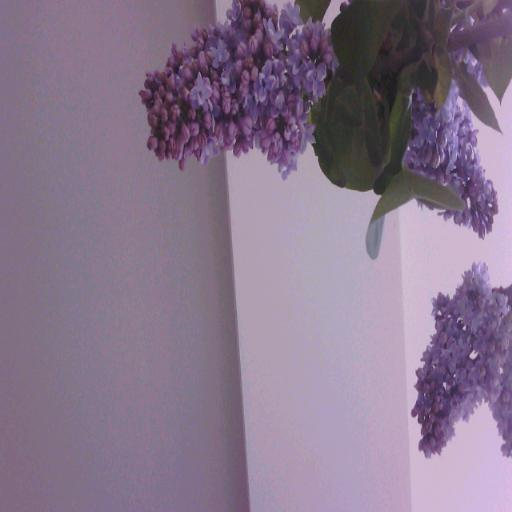
\includegraphics[width=\linewidth]{figures/experiment_frames/fig_scene_cam0.jpg}
\caption{cam0 (front, rotated 180°)}
\label{fig:scene:cam0}
\end{subfigure}\hfill
\begin{subfigure}[t]{0.44\linewidth}
\centering
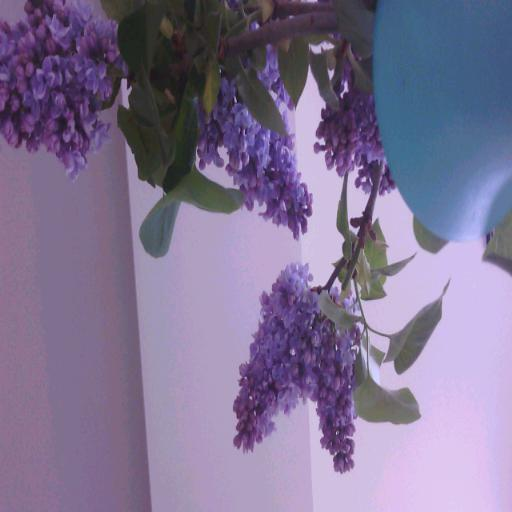
\includegraphics[width=\linewidth]{figures/experiment_frames/fig_scene_cam1.jpg}
\caption{cam1 (back, unrotated)}
\label{fig:scene:cam1}
\end{subfigure}
\caption{Canonical scene used throughout every E15–E18 measurement.
Two lilac arrangements against a pale wall, with a teal ceramic mug
in the upper right of cam0's field of view.  Both images are 512×512
JPEG quality-75 captured by the on-board PXP pipeline at the start
of session \texttt{s045\_e18\_post\_refactor} / \texttt{s044\_e18\_headtail\_drain2}.
The scene contains no instances of the model's target class, so every
measured frame has \texttt{num\_detections == 0} — an explicit design
choice that isolates timing from detection-count variance.}
\label{fig:scene}
\end{figure}

\begin{center}\rule{0.5\linewidth}{0.5pt}\end{center}

\section{6. Measurement tooling}\label{measurement-tooling}

\subsection{\texorpdfstring{6.1 On-device: the \texttt{diag}
package}{6.1 On-device: the diag package}}\label{on-device-the-diag-package}

Experiments are implemented as Python functions in
\texttt{examples/sentai\_runtime/diag/}, invoked from the REPL as
\texttt{diag.eN\_xxx(...)}. Each function:

\begin{itemize}
\tightlist
\item
  Opens (or inherits) a session
\item
  Sets a known firmware state (\texttt{verbose(0)}, \texttt{ratio(0,0)},
  \texttt{switch\_drain(2)}, pipeline stopped, \texttt{gc.collect()})
\item
  Runs a warm-up block
\item
  Executes N timed iterations, dropping the first
\item
  Writes \texttt{NNN\_\textless{}name\textgreater{}.csv} +
  \texttt{NNN\_\textless{}name\textgreater{}.txt} + records in
  \texttt{manifest.csv}
\item
  Returns a summary dict
\end{itemize}

A list of experiment functions relevant to the performance story:

{\def\LTcaptype{none} % do not increment counter
\begin{longtable}[]{@{}
  >{\raggedright\arraybackslash}p{(\linewidth - 4\tabcolsep) * \real{0.3333}}
  >{\raggedright\arraybackslash}p{(\linewidth - 4\tabcolsep) * \real{0.3333}}
  >{\raggedright\arraybackslash}p{(\linewidth - 4\tabcolsep) * \real{0.3333}}@{}}
\toprule\noalign{}
\begin{minipage}[b]{\linewidth}\raggedright
ID
\end{minipage} & \begin{minipage}[b]{\linewidth}\raggedright
Function
\end{minipage} & \begin{minipage}[b]{\linewidth}\raggedright
What it measures
\end{minipage} \\
\midrule\noalign{}
\endhead
\bottomrule\noalign{}
\endlastfoot
E13 & \texttt{e13\_pipeline\_full} & Sequential pipeline at 320×320,
per-stage timing \\
E14 & \texttt{e14\_pipeline\_parallel} &
\texttt{sentai.pipeline.start/get/stop} throughput (parallel
\texttt{PrepTask\ +\ InferTask}) \\
E15 & \texttt{e15\_pipeline\_parallel\_512} & E14 wrapper for the
512×512 1-class model \\
E16 & \texttt{e16\_camera\_switch\_512} & Alternating cam0↔cam1
sequential, per-stage timing \\
E17 & \texttt{e17\_switch\_drain\_visual} & Per-switch JPEG capture
(in-RAM buffer; LFS write deferred so timing is clean) \\
E18 & \texttt{e18\_camera\_switch\_headtail} & Three-sweep benchmark in
one session: fixed cam0, fixed cam1, alternating \\
\end{longtable}
}

\subsection{6.2 Time source}\label{time-source}

\texttt{sentai.rtos.ticks\_ms()} --- FreeRTOS tick counter exposed to
MicroPython. Resolution 1 ms, wrap at 49.7 days (handled by delta
subtraction). All stage timings are either this counter (host- visible)
or the firmware's own wrapper around its invoke duration (returned as
the integer ms value of \texttt{sentai.tpu.invoke()}).

\subsection{6.3 Statistical tools}\label{statistical-tools}

Means, stdev (Bessel-corrected), min/max, median are computed offline
from the raw CSVs by the appendix generator
\href{../experiments/_build_appendix.py}{\texttt{experiments/\_build\_appendix.py}}.
The device never reports a summary statistic except the short
\texttt{"mean=X\ fps=Y"} string in each manifest row, and that is
informational only --- the numbers that appear in paper tables are
always re-derived from the raw per-iteration CSVs.

See \href{../experiments/methodology.md}{experiments/methodology.md} for
the full protocol (warm-up drop, repetition count rationale,
reproducibility criteria, noise budget). The short form is: every
reported number is the mean of n ≥ 19 independent iterations with the
first sample dropped; sessions are self-contained; the same scene,
model, and firmware build underlie any cross-session comparison.

\begin{center}\rule{0.5\linewidth}{0.5pt}\end{center}

\section{7. Host environment}\label{host-environment}

{\def\LTcaptype{none} % do not increment counter
\begin{longtable}[]{@{}
  >{\raggedright\arraybackslash}p{(\linewidth - 2\tabcolsep) * \real{0.5000}}
  >{\raggedright\arraybackslash}p{(\linewidth - 2\tabcolsep) * \real{0.5000}}@{}}
\toprule\noalign{}
\begin{minipage}[b]{\linewidth}\raggedright
Component
\end{minipage} & \begin{minipage}[b]{\linewidth}\raggedright
Value
\end{minipage} \\
\midrule\noalign{}
\endhead
\bottomrule\noalign{}
\endlastfoot
OS & Linux 6.17 (kernel), Ubuntu-derived userland \\
USB stack & \texttt{cdc\_acm} + \texttt{cdc\_ncm} kernel modules, MSC
via \texttt{littlefs-fuse} \\
IP & USB-NCM: host \texttt{10.0.0.N/24}, device \texttt{10.0.0.1} \\
Python & 3.12, \texttt{pyserial} for REPL-driven uploads \\
Build & CMake 3.x + Ninja/Make, arm-none-eabi-gcc 10+ \\
Firmware flash &
\texttt{python3\ scripts/flashtool.py\ -e\ sentai\_runtime} \\
Result fetch & HTTP GET from \texttt{http://10.0.0.1/api/raw/diags/…}
with \texttt{lfs\_busy} retry \\
\end{longtable}
}

The exact host details matter only insofar as they influence measurement
access (e.g.~the REPL-chunked uploader at
\href{../diag/_host_upload_repl.py}{\texttt{diag/\_host\_upload\_repl.py}}
exists because HTTP POST to \texttt{/api/write/} hangs on this
firmware). None of the performance numbers reported in this paper depend
on host scheduling or host I/O; they are all measured on-device and
fetched post-hoc.

\begin{center}\rule{0.5\linewidth}{0.5pt}\end{center}

\section{8. Summary of what changes between experiments, and what does
not}\label{summary-of-what-changes-between-experiments-and-what-does-not}

A reader comparing two sessions should know that the following are
\textbf{held constant} across every E15-E18 result in this paper unless
a section explicitly notes a departure:

\begin{itemize}
\tightlist
\item
  Hardware (same SentAI board unit, no swap of camera modules, no
  physical rework)
\item
  OV5640 PLL and sensor-init register sequences (same NXP driver lookup)
\item
  Scene (static lilac arrangement, no lighting changes)
\item
  Model (\texttt{yolo\_1\_class\_512\_…\_P5\_32.tflite}, compiled for
  EdgeTPU Mode

  \begin{enumerate}
  \def\labelenumi{\arabic{enumi})}
  \setcounter{enumi}{2}
  \tightlist
  \item
  \end{enumerate}
\item
  Logical resolution requested (512×512 unless the section says VGA or
  QVGA)
\item
  Warm-up protocol (one full cycle per camera before the measured loop)
\item
  Warm-up sample drop (first measurement sample discarded from stats)
\item
  Fault-counter check (post-run \texttt{sentai.diag.cam\_stats()} values
  are recorded; a non-zero degraded-path counter invalidates a session)
\end{itemize}

What \emph{does} change between the sessions the paper compares:

\begin{itemize}
\tightlist
\item
  The firmware build (documented per-section in the cross-session
  comparison tables --- e.g.~\url{cam_switch.md} §``Cross- session
  comparison'')
\item
  The A/B runtime flag under test (\texttt{dma\_memcpy(0/1)},
  \texttt{switch\_drain(1/2)}, \texttt{ratio(0,0)\ /\ (3,1)\ /\ (9,1)})
\item
  The chosen alternation pattern (fixed cam0, fixed cam1, or alternating
  --- the three sweeps of E18)
\end{itemize}

A reviewer verifying a specific claim can thus navigate directly: the
numeric claim → the section that presents it → the session name → the
folder under \href{../experiments/}{\texttt{../experiments/}} with the
raw CSV. The claim-to-file mapping is tabulated in \url{artifact.md}.
